\subsection{Arten}

Der wichtigste und komplizierteste Teil beim maschinellem Lernen ist die Kunst einem Computer das selbständige Lernen beizubringen, dabei orientiert man sich am Lernprozess eines Menschen. Dazu besteht es eine Vielzahl an Ansätzen und zu den bekanntesten gehören:

\begin{itemize}
    \item Supervised Learning
    \item Unsupervised Learning
    \item Reinforcement Learning
\end{itemize}

Um diese Ansätze nachvollziehen zu können, muss man zuerst die menschliche Intelligenz verstehen, oder genauer gesagt die Frage ''Wie lernt das menschliche Gehirn?''.

\subsubsection{Menschliche Ürsprünge vom Machine Learning}

Bereits als Fötus entwickeln sich Neuronen, die sich über die Zeit verknüpfen und gemeinsam ein Netzwerk bilden, welches dem Körper Anweisungen übermittelt. Daher kommt ein Neugeborenes mit etwa 100 Milliarden Neuronen auf die Welt, die zur Zeit der Geburt nur schwach miteinander verbunden sind. Mithilfe des Lernens werden diese Verbindungen gestärkt und das Kind kann Vorgehensweisen besser verstehen und neue Erkenntnisse gewinnen, damit steigt zusätzlich auch das Gewicht und die Größe des Gehirnes. \cite{LANP}

Jedoch verschwinden diese Verbindungen, falls sie nicht aufgefrischt werden und Informationen in Vergessenheit verfallen. Weitere Faktoren könnte der Alterungsprozess oder eine neurologische Krankheit sein, die das Phänomen erklären, dass man im höheren Alter Probleme beim Lernen hat. \cite{GENTW}

\begin{figure}[H]
    \centering
    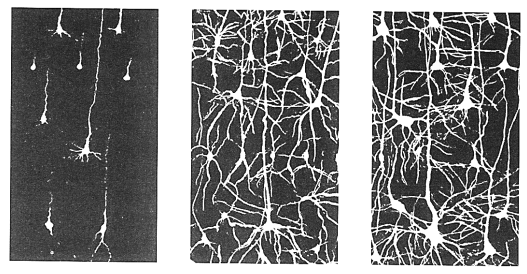
\includegraphics[scale=0.8]{sections/machine-learning/images/neuronale-netze.png}
    \caption{Vernetzungen nach der Geburt, nach 3 Monaten und nach 15 Monaten}
\end{figure}
%https://www.uni-wuerzburg.de/fileadmin/06000060/04_Fort-_und_Weiterbildungen_Lehrkraefte/Herbsttagungen/Herbsttagung_2016/20161006_WS_04_Neurobiologie.pdf

Neue Informationen verbinden bereits bestehende Neuronen und altes Wissen wird erneuert. Außerdem wird mit oftmaligem Wiederholen das Netzwerk dichter und man kann das Erlernte leichter abrufen, zugleich werden die neuen Informationen mit dem bereits existierenden Vorwissen besser kombiniert. \cite{LANP}

\subsubsection{Supervised Learning}

An einen Algorithmus werden gruppierte Daten übergeben, die neben einer Gruppe noch mehrere Merkmale beinhalten, um danach neue Datensätze zu klassifizieren oder zu regredieren. Die Bezeichnung ''Supervised'' (im Deutschen ''Überwachtes'') kommt daher, dass die Gruppen bereits vordefiniert sind und das Programm nicht selber welche erstellen muss. \cite{SL:online}

\begin{table}[H]
    \centering
    \resizebox{.7\textwidth}{!}{
        \begin{tabular}{|l|l|l|l|}
            \hline
            \textbf{Farbe} & \textbf{Form} & \textbf{Geschmack} & \textbf{Frucht} \\ \hline
            rot            & herzförmig    & süß                & Erdbeere        \\ \hline
            gelb           & oval          & säuerlich          & Zitrone         \\ \hline
            rot            & rund          & süß                & Apfel           \\ \hline
            grün           & rund          & säuerlich          & Apfel           \\ \hline
        \end{tabular}}
    \caption{Beispiel für gruppierte Daten als Tabelle; Merkmale: Farbe, Form, Geschmack; Gruppe: Frucht}
    \label{tbl:fruit-data}
\end{table}

Diese Art von Lernen kann man in zwei Typen aufteilen:

\begin{itemize}
    \item Klassifizierung
    \item Regression
\end{itemize}

\paragraph{Klassifizierungs} Probleme verwenden Algorithmen, um Daten einer bestimmten Kategorie zuzuteilen. Oft gibt es nur zwei Kategorien wie zum Beispiel Hund/Katze oder Ja/Nein, jedoch gibt es auch Fälle wo eine Vorhersage mit einer Wahrscheinlichkeit zwischen 0 und 1 getroffen wird. Weiteres gibt es auch Situationen, wo zwischen einer großen Menge an Kategorien ausgewählt wird, zum Beispiel bei der Erkennung von handschriftlichen Ziffern, in diesem Beispiel würde es zehn Möglichkeiten geben.

\begin{figure}[H]
    \centering
    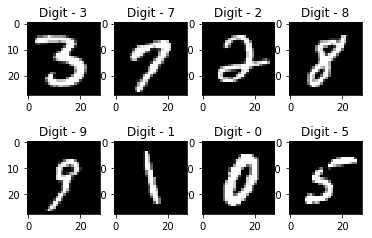
\includegraphics{sections/machine-learning/images/0_8-vKSQnZvKbtKXKy.png}
    \caption{Beispiel für eine Klassifizierung von handschriftlichen Ziffern}
    \label{ziffern}
\end{figure}
% https://aleenamishra10.medium.com/handwritten-digit-recognition-using-machine-learning-f6a08761ff83

Zu diesen ''überwachten'' Algorithmen gehören Lineare Diskriminanzanalysen, Support Vector Machines (SVM), Random Forests und Entscheidungsbäume \cite{SL:online}.

\subparagraph{Entscheidungsbäume} (Decision Trees) sind eine hierarchische Abfolge von Bedingungen und sind vergleichbar mit verschachtelten if/else-Statements. Dabei beginnt der Entscheidungsbaum mit einer Bedingung, die auch als ''Root-Node'' bezeichnet wird, worauf im Normalfall weitere Bedingungen folgen. Die Blätter dieser Pfade spiegeln die Gruppen oder Klassifizierungen wieder und sind nur über mehrere Pfade erreichbar.

Jedoch haben ein Entscheidungsbäume das Problem, dass sie sehr gut mit den antrainierten Daten arbeiten und weniger genau mit neuen Daten (Overfitting \ref{overfitting}). Um diese Genauigkeit zu verbessern kann man zum Beispiel über Hyperparameter die maximale Länge eines Pfades setzen, wodurch die Bedingungen verallgemeinert werden.

\begin{figure}[H]
    \centering
    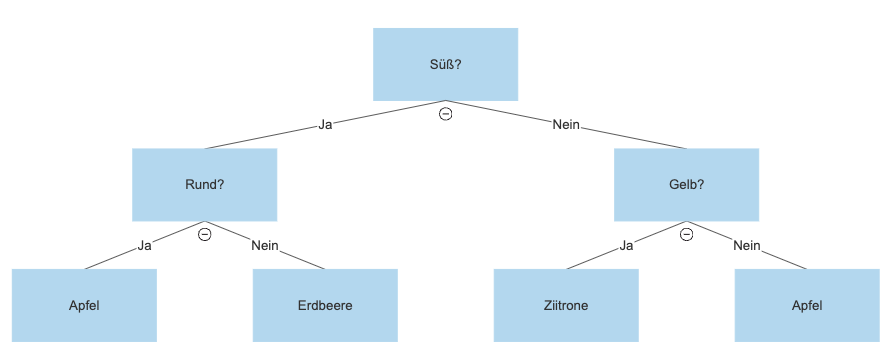
\includegraphics[scale=0.5]{sections/machine-learning/images/decision-tree.png}
    \caption{Decision Tree an dem Beispiel von Tabelle \ref{tbl:fruit-data}}
\end{figure}

In diesem Beispiel sieht dieser Entscheidungsbaum noch sehr lesbar aus, jedoch ändert sich dies, wenn Entscheidungen dargestellt werden, bei denen es auf die Nachkommastelle ankommt und wenn die Kategorien sehr schwer differenzierbar sind. Bei dem Supervised Learning erstellt das Programm selbstständig einen Entscheidungsbaum, indem es Muster oder Zusammenhänge findet und analysiert. Nach vielem Lernen kann dieser Entscheidungsbaum optimiert werden und unnötige Verbindungen können entfernt werden.

Fast man mehrere Entscheidungsbäume zusammen, entsteht ein Random Forest, wobei jeder Entscheidungsbaum nur bestimmte Spalten/Merkmale zugeteilt bekommt. Soll ein neuer Datensatz kategorisiert werden, entscheidet die Mehrheit der jener Ergebnisse der Entscheidungsbäume, zu welcher Gruppe dieser Datensatz dazugehört.

\paragraph{Regressionen,} Erstellung einer kontinuierlichen Funktion mithilfe von Werten, die auf oder nahe an der Funktion liegen, sind hilfreich, wenn anstatt diskreten Werten kontinuierliche Werte, wie zum Beispiel die Größe einer Person, festgestellt werden sollen. Dazu gehören lineare Regressionen und polynominale Regression.

\subsubsection{Unsupervised Learning}

Beim Unsupervised Learning, oder unüberwachtes Lernen, werden Verbindungen ohne genauere Informationen über den Testdatensatz erzeugt. Dabei muss das Programm selbst Gruppen definieren und dann die übergebenen Daten in diese Gruppen zuordnen. \cite{SL:online}

\paragraph{Clustering} gehört zu den beliebtesten Varianten, um selbstständig Gruppen zu erstellen. Dabei wird jeder Datensatz als Punkt in ein Koordinatensystem mit beliebig vielen Dimensionen eingetragen. Eine Achse stellt ein Attribut dar und je nach Ausprägung ist der Punkt mehr oder weniger vom Ursprung entfernt.

\begin{figure}[H]
    \centering
    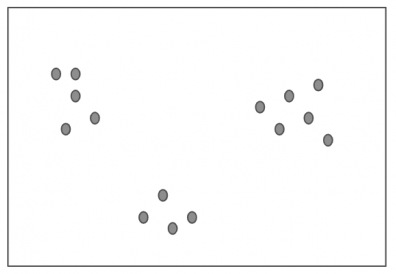
\includegraphics[scale=0.8]{sections/machine-learning/images/unclustered-data.png}
    \caption{Unkategorisierte Daten}
    \label{fig:unclustered-data}
\end{figure}
%https://datascience.eu/de/maschinelles-lernen/clustering-algorithmen-und-ihre-bedeutung-beim-maschinellen-lernen-2/

Auch für das menschliche Auge ist es möglich dieses Beispiel (Abbildung \ref{fig:unclustered-data}) in Haufen oder Klumpen zusammenzufassen, genau das gleiche macht ein Programm mit Clustern. Die Interpretation dieser Gruppen muss jedoch wieder durch Menschen erfolgen, da ein Computer nicht im Stande dazu ist, dieser Cluster einer Kategorie zuzuteilen.

Diese Vorgehensweise wird oft in sehr komplizierte Einsatzbereiche genutzt, und daher ist es sehr schwer differenzierbare Cluster zu erstellen. Der Prozess, solche Cluster zu definieren, basiert darauf, die Punkte so zu gruppieren, dass der Abstand in diesem Cluster klein ist und zu anderen Clustern groß.

\begin{figure}[H]
    \centering
    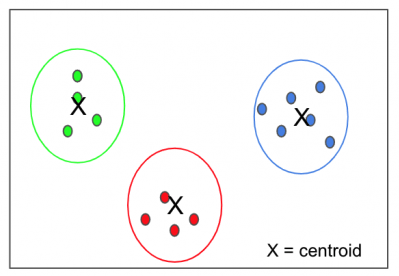
\includegraphics[scale=0.8]{sections/machine-learning/images/clustered-data.png}
    \caption{Kategorisierte Daten}
    \label{fig:clustered-data}
\end{figure}

\subsubsection{Reinforcement Learning}

Das Reinforcement Learning, oder das beschränkte/verstärkte Lernen, wird oft mit dem Konzept ''Learning by doing'' verglichen, da es sich weniger auf das Ergebnis fokussiert und mehr auf Aktionen oder Vorgängen. Ein Beispiel für diese Vorgehensweise aus der Sicht eines Schülers ist das Üben vor einer Matheschularbeit. Wird während dem Üben ein Fehler gemacht, merkt man sich das Problem und passt sein Verhalten / seinen Rechenweg so an, dass dieser Fehler nicht mehr vorkommt. Die nennt man auch negative Verstärkung. \cite{SL:online}

Dahingegen führen richtige Ergebnisse oder erwarteten Reaktionen zu positiven Verstärkungen und man versucht dieses Verhalten zu wiederholen.

Durch negative und positive Verstärkungen wird das Verhalten verbessert, um den besten Weg zum Ziel zu finden. Bei komplexen Systemen kann dies selbstständig vom Programm gemacht werden, jedoch bei simpleren kann es geschehen, dass ein unnötig komplizierter Weg gefunden wird. In diesen Fällen schaut ein Supervisor dem Programm ''über die Schulter''.